% Preamble templated from Dhawal24112006/EE1030
\documentclass{beamer}
\mode<presentation>
\usepackage{amsmath}
\usepackage{amssymb}
%\usepackage{advdate}
\usepackage{adjustbox}
\usepackage{subcaption}
% \usepackage{enumitem}
\usepackage{multicol}
\usepackage{mathtools}
\usepackage{listings}
\usepackage{url}
% \usepackage{../gvv}
\def\UrlBreaks{\do\/\do-}
\usetheme{Boadilla}
\usecolortheme{lily}
\setbeamertemplate{footline}
{
  \leavevmode%
  \hbox{%
  \begin{beamercolorbox}[wd=\paperwidth,ht=2.25ex,dp=1ex,right]{author in head/foot}%
    \insertframenumber{} / \inserttotalframenumber\hspace*{2ex}
  \end{beamercolorbox}}%
  \vskip0pt%
}
\setbeamertemplate{navigation symbols}{}

\providecommand{\nCr}[2]{\,^{#1}C_{#2}} % nCr
\providecommand{\nPr}[2]{\,^{#1}P_{#2}} % nPr
\providecommand{\mbf}{\mathbf}
\providecommand{\pr}[1]{\ensuremath{\Pr\left(#1\right)}}
\providecommand{\qfunc}[1]{\ensuremath{Q\left(#1\right)}}
\providecommand{\sbrak}[1]{\ensuremath{{}\left[#1\right]}}
\providecommand{\lsbrak}[1]{\ensuremath{{}\left[#1\right.}}
\providecommand{\rsbrak}[1]{\ensuremath{{}\left.#1\right]}}
\providecommand{\brak}[1]{\ensuremath{\left(#1\right)}}
\providecommand{\lbrak}[1]{\ensuremath{\left(#1\right.}}
\providecommand{\rbrak}[1]{\ensuremath{\left.#1\right)}}
\providecommand{\cbrak}[1]{\ensuremath{\left\{#1\right\}}}
\providecommand{\lcbrak}[1]{\ensuremath{\left\{#1\right.}}
\providecommand{\rcbrak}[1]{\ensuremath{\left.#1\right\}}}
\theoremstyle{remark}
\newtheorem{rem}{Remark}
\newcommand{\sgn}{\mathop{\mathrm{sgn}}}
\providecommand{\abs}[1]{\left\vert#1\right\vert}
\providecommand{\res}[1]{\Res\displaylimits_{#1}}
\providecommand{\norm}[1]{\lVert#1\rVert}
\providecommand{\mtx}[1]{\mathbf{#1}}
\providecommand{\mean}[1]{E\left[ #1 \right]}
\providecommand{\fourier}{\overset{\mathcal{F}}{ \rightleftharpoons}}
%\providecommand{\hilbert}{\overset{\mathcal{H}}{ \rightleftharpoons}}
\providecommand{\system}{\overset{\mathcal{H}}{ \longleftrightarrow}}
	%\newcommand{\solution}[2]{\textbf{Solution:}{#1}}
%\newcommand{\solution}{\noindent \textbf{Solution: }}
\providecommand{\dec}[2]{\ensuremath{\overset{#1}{\underset{#2}{\gtrless}}}}
\newcommand{\myvec}[1]{\ensuremath{\begin{pmatrix}#1\end{pmatrix}}}
\newcommand{\augvec}[3]{\ensuremath{\begin{amatrix}{#1|#2}#3\end{amatrix}}}
\NewDocumentEnvironment{amatrix}{>{\SplitArgument{1}{|}}m}
 {\left(\makeamatrix#1}
 {\end{array}\right)}
\NewDocumentCommand{\makeamatrix}{mm}{%
  \IfNoValueTF{#2}
    {\begin{array}{@{}*{#1}{c}@{}}}
    {\begin{array}{@{}*{#1}{c}|*{#2}{c}@{}}}%
}
\let\vec\mathbf

\lstset{
%language=C,
frame=single,
breaklines=true,
columns=fullflexible,
showstringspaces=false
}

\numberwithin{equation}{section}

\title{MATGEO Presentation: 5.5.7}
\author{Subhodeep Chakraborty \\ ee25btech11055,\\IIT Hyderabad.}

\date{\today}
\begin{document}

\begin{frame}
\titlepage
\end{frame}

\section*{Outline}
\begin{frame}
\tableofcontents
\end{frame}

\section{Problem}
\begin{frame}
\frametitle{Problem Statement}

Find the inverse of the following matrix, using elementary transformations\hfill\brak{12, 2019}
$$\myvec{2&3&1\\2&4&1\\3&7&2}$$
\end{frame}

\section{Solution}
\begin{frame}{Given data}
Given:
\begin{align}
 \vec{A} = \myvec{2&3&1\\2&4&1\\3&7&2}
\end{align}
\end{frame}

\begin{frame}{Formulae}
Let $\vec{A^{-1}}$ be inverse of $\vec{A}$
We know \begin{align}\vec{A}\vec{A^{-1}} = \vec{I}\end{align}
Thus augmented matrix to find $\vec{A^{-1}}$ is given by: $\augvec{1}{1}{\vec{A}&\vec{I}}$
\end{frame}

\begin{frame}{Solving}
\begin{align}
\augvec{3}{3}{2&3&1&1&0&0\\2&4&1&0&1&0\\3&7&2&0&0&1} \xleftrightarrow[]{R1 \xleftrightarrow[]{} R3; R1 = R1/3}& \\
\augvec{3}{3}{1&7/3&2/3&0&0&1/3\\2&4&1&0&1&0\\2&3&1&1&0&0} \xleftrightarrow[]{R2=R2-2R1;R3=R3-2R1}& \\
\augvec{3}{3}{1&7/3&2/3&0&0&1/3\\0&-2/3&-1/3&0&1&-2/3\\0&-5/3&-1/3&1&0&-2/3} \xleftrightarrow[]{R3=-5/3R3}& \\
\augvec{3}{3}{1&7/3&2/3&0&0&1/3\\0&-2/3&-1/3&0&1&-2/3\\0&1&1/5&-3/5&0&2/5} \xleftrightarrow[]{R1 = R1-7/3R3; R2 = 2/3R3}& \\
\augvec{3}{3}{1&0&1/5&7/5&0&-3/5\\0&0&-1/5&-2/5&1&-2/5\\0&1&1/5&-3/5&0&2/5} \xleftrightarrow[]{R2\xleftrightarrow[]{}R3}& \\
\augvec{3}{3}{1&0&1/5&7/5&0&-3/5\\0&1&1/5&-3/5&0&2/5\\0&0&-1/5&-2/5&1&-2/5} \xleftrightarrow[]{R1=R1+R3;R2=R2-R3}&
\augvec{3}{3}{1&0&0&1&1&-1\\0&1&0&-1&1&0\\0&0&1&2&-5&2}
\end{align}
\end{frame}
\begin{frame}{Result}
So we have:
\begin{align}
 \vec{A^{-1}}=\myvec{1&1&-1\\-1&1&0\\2&-5&2}
\end{align}
\end{frame}
\subsection{Plot}
\begin{frame}{Plot}
 \begin{figure}[H]
    \centering
    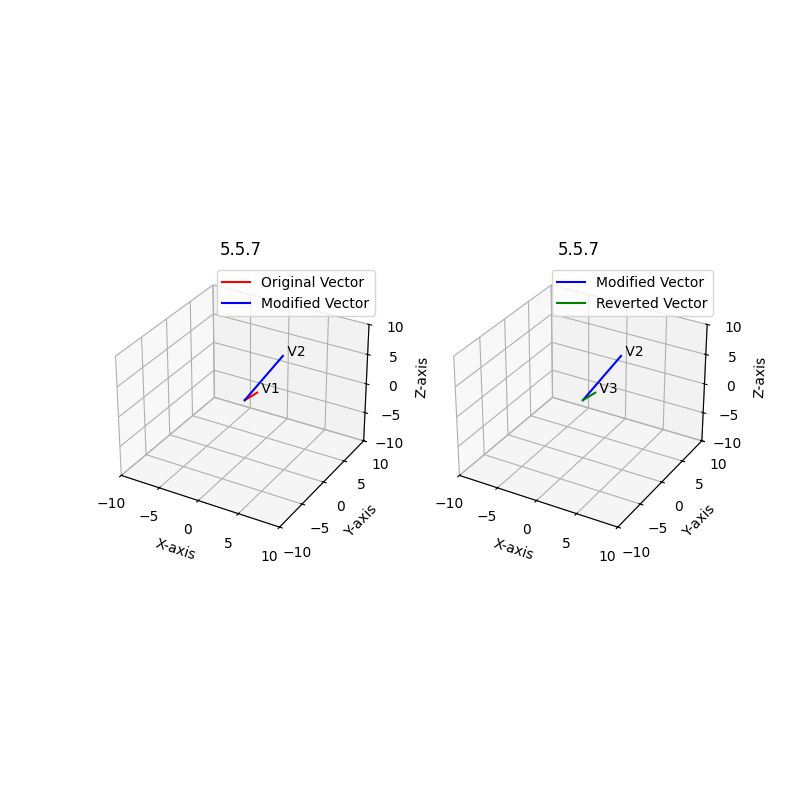
\includegraphics[width=0.8\columnwidth]{../figs/plot.png}
    \caption*{}
    \label{fig:plot}
\end{figure}
\end{frame}

\section{C Code}

\begin{frame}[fragile]{C code for generating points on line}
\begin{lstlisting}[language=C]
void point_gen(const double* P1, const double* P2, double t, double* result_point) {
    result_point[0] = P1[0] + t * (P2[0] - P1[0]);
    result_point[1] = P1[1] + t * (P2[1] - P1[1]);
    result_point[2] = P1[2] + t * (P2[2] - P1[2]);
}
\end{lstlisting}
\end{frame}
\begin{frame}[fragile]{C Code for matrix functions}
 \begin{lstlisting}[language=C]
#include <stdio.h>
#include <stdlib.h>
#include <math.h>

int find_inverse(const double *input_matrix, double *inverse_matrix, int n) {
    // Read up on memory
    double *augmented = (double *)malloc(n * 2 * n * sizeof(double));

    int i, j, k;
    const int width = 2 * n;
\end{lstlisting}
\end{frame}
\begin{frame}[fragile]
\begin{lstlisting}[language=C]
    for (i = 0; i < n; ++i) {
        for (j = 0; j < n; ++j) {
            augmented[i * width + j] = input_matrix[i * n + j];
        }
        for (j = n; j < width; ++j) {
            augmented[i * width + j] = (i == (j - n)) ? 1.0 : 0.0;
        }
    }

    for (i = 0; i < n; ++i) {
        // check why this matters. smtg to do with errors sir said iirc
        int max_row = i;
        for (k = i + 1; k < n; ++k) {
            if (fabs(augmented[k * width + i]) > fabs(augmented[max_row * width + i])) {
                max_row = k;
            }
        }
\end{lstlisting}
\end{frame}
\begin{frame}[fragile]
\begin{lstlisting}[language=C]
        if (max_row != i) {
            for (k = 0; k < width; ++k) {
                double temp = augmented[i * width + k];
                augmented[i * width + k] = augmented[max_row * width + k];
                augmented[max_row * width + k] = temp;
            }
        }

        // check singular
        if (fabs(augmented[i * width + i]) < 1e-9) {
            free(augmented);
            return 0;
        }
\end{lstlisting}
\end{frame}
\begin{frame}[fragile]
\begin{lstlisting}[language=C]
        // -make 1
        double pivot = augmented[i * width + i];
        for (j = i; j < width; ++j) {
            augmented[i * width + j] /= pivot;
        }

        // make zero
        for (j = 0; j < n; ++j) {
            if (i != j) {
                double factor = augmented[j * width + i];
                for (k = 0; k < width; ++k) {
                    augmented[j * width + k] -= factor * augmented[i * width + k];
                }
            }
        }
    }
\end{lstlisting}
\end{frame}
\begin{frame}[fragile]
\begin{lstlisting}[language=C]
    // Output inverse
    for (i = 0; i < n; ++i) {
        for (j = 0; j < n; ++j) {
            inverse_matrix[i * n + j] = augmented[i * width + (j + n)];
        }
    }

    free(augmented);
    return 1;
}
\end{lstlisting}
\end{frame}
\begin{frame}[fragile]
\begin{lstlisting}[language=C]
void mul(const double *a, const double *b, double *c, int m, int n, int p) {
    for (int i = 0; i < m; i++) {
        for (int k = 0; k < p; k++) {
            double temp = 0.0;
            for (int j = 0; j < n; j++) {
                temp += a[i * n + j] * b[j * p + k];
            }
            c[i * p + k] = temp;
        }
    }
}

 \end{lstlisting}
\end{frame}

\section{Python Code}
\subsection{Using shared objects}
\begin{frame}[fragile]{Python code for plotting using C}
\begin{lstlisting}[language=Python]
import ctypes
import numpy as np
import numpy.linalg as LA
import matplotlib.pyplot as plt
import sys

libline = ctypes.CDLL("./line.so")
get_point = libline.point_gen
get_point.argtypes = [
    ctypes.POINTER(ctypes.c_double),  # P1
    ctypes.POINTER(ctypes.c_double),  # P2
    ctypes.c_double,  # t
    ctypes.POINTER(ctypes.c_double),  # result_point
]
get_point.restype = None
\end{lstlisting}
\end{frame}
\begin{frame}[fragile]
\begin{lstlisting}[language=Python]
libmatrix = ctypes.CDLL("./matrix.so")
libmatrix.find_inverse.argtypes = [
    np.ctypeslib.ndpointer(dtype=np.float64, ndim=1, flags="C_CONTIGUOUS"),
    np.ctypeslib.ndpointer(dtype=np.float64, ndim=1, flags="C_CONTIGUOUS"),
    ctypes.c_int,
]
libmatrix.find_inverse.restype = ctypes.c_int
find_inv = libmatrix.find_inverse
\end{lstlisting}
\end{frame}
\begin{frame}[fragile]
\begin{lstlisting}[language=Python]
libmatrix.mul.argtypes = [
    np.ctypeslib.ndpointer(dtype=np.float64, ndim=1, flags="C_CONTIGUOUS"),
    np.ctypeslib.ndpointer(dtype=np.float64, ndim=1, flags="C_CONTIGUOUS"),
    np.ctypeslib.ndpointer(dtype=np.float64, ndim=1, flags="C_CONTIGUOUS"),
    ctypes.c_int,
    ctypes.c_int,
    ctypes.c_int,
]
libmatrix.mul.restype = None
matmul = libmatrix.mul
\end{lstlisting}
\end{frame}
\begin{frame}[fragile]
\begin{lstlisting}[language=Python]
DoubleArray3 = ctypes.c_double * 3
a = DoubleArray3(0,0,0)
x = np.array([1,1,1],dtype=np.float64)

A = np.array([[3, 0, -1], [2, 3, 0], [0, 4, 1]],dtype=np.float64)
A_flat = A.flatten()
# flatten() passes a COPY! matrix isn't stored
inv = np.empty_like(A_flat)
if not find_inv(A_flat,inv,3):
    print("Matrix is singular")
    sys.exit()

inv = inv.reshape(A.shape)
b = np.empty_like(x)
c = np.empty_like(x)
matmul(A.flatten(),x,b,3,3,1)
matmul(inv.flatten(),b,c,3,3,1)
\end{lstlisting}
\end{frame}
\begin{frame}[fragile]
\begin{lstlisting}[language=Python]
fig = plt.figure(figsize=(8, 8))
ax = fig.add_subplot(121, projection="3d")

t_values = np.linspace(0, 1, 100)
line_points_x, line_points_y, line_points_z = [], [], []
for t in t_values:
    result_arr = DoubleArray3()
    get_point(a, DoubleArray3(x[0], x[1], x[2]), t, result_arr)
    line_points_x.append(result_arr[0])
    line_points_y.append(result_arr[1])
    line_points_z.append(result_arr[2])
ax.plot(
    line_points_x,
    line_points_y,
    line_points_z,
    color="red",
    label="Original Vector"
)
ax.text(x[0], x[1], x[2], " V1")
\end{lstlisting}
\end{frame}
\begin{frame}[fragile]
\begin{lstlisting}[language=Python]
t_values = np.linspace(0, 1, 100)
line_points_x, line_points_y, line_points_z = [], [], []

for t in t_values:
    result_arr = DoubleArray3()

    get_point(a, DoubleArray3(b[0], b[1], b[2]), t, result_arr)

    line_points_x.append(result_arr[0])
    line_points_y.append(result_arr[1])
    line_points_z.append(result_arr[2])
ax.plot(
    line_points_x,
    line_points_y,
    line_points_z,
    color="blue",
    label="Modified Vector"
)
ax.text(b[0], b[1], b[2], " V2")
\end{lstlisting}
\end{frame}
\begin{frame}[fragile]
\begin{lstlisting}[language=Python]
ax2 = fig.add_subplot(122, projection="3d")

t_values = np.linspace(0, 1, 100)
line_points_x, line_points_y, line_points_z = [], [], []
for t in t_values:
    result_arr = DoubleArray3()
    get_point(a, DoubleArray3(b[0], b[1], b[2]), t, result_arr)
    line_points_x.append(result_arr[0])
    line_points_y.append(result_arr[1])
    line_points_z.append(result_arr[2])
ax2.plot(
    line_points_x,
    line_points_y,
    line_points_z,
    color="blue",
    label="Modified Vector"
)
ax2.text(b[0], b[1], b[2], " V2")
\end{lstlisting}
\end{frame}
\begin{frame}[fragile]
\begin{lstlisting}[language=Python]
t_values = np.linspace(0, 1, 100)
line_points_x, line_points_y, line_points_z = [], [], []

for t in t_values:
    result_arr = DoubleArray3()

    get_point(a, DoubleArray3(c[0], c[1], c[2]), t, result_arr)

    line_points_x.append(result_arr[0])
    line_points_y.append(result_arr[1])
    line_points_z.append(result_arr[2])
ax2.plot(
    line_points_x,
    line_points_y,
    line_points_z,
    color="green",
    label="Reverted Vector"
)
ax2.text(c[0], c[1], c[2], " V3")
\end{lstlisting}
\end{frame}
\begin{frame}[fragile]
\begin{lstlisting}[language=Python]
ax.set_xlabel("X-axis")
ax.set_ylabel("Y-axis")
ax.set_zlabel("Z-axis")
ax.set_title("5.5.7")
ax.set_xlim([-10, 10])
ax.set_ylim([-10, 10])
ax.set_zlim([-10, 10])
ax.legend()
ax.grid(True)
ax2.set_xlabel("X-axis")
ax2.set_ylabel("Y-axis")
ax2.set_zlabel("Z-axis")
ax2.set_title("5.5.7")
ax2.set_xlim([-10, 10])
ax2.set_ylim([-10, 10])
ax2.set_zlim([-10, 10])
ax2.legend()
ax2.grid(True)
plt.savefig("../figs/plot.png")
plt.show()
\end{lstlisting}
\end{frame}

\subsection{Plot}
\begin{frame}{Plot}
 \begin{figure}[H]
    \centering
    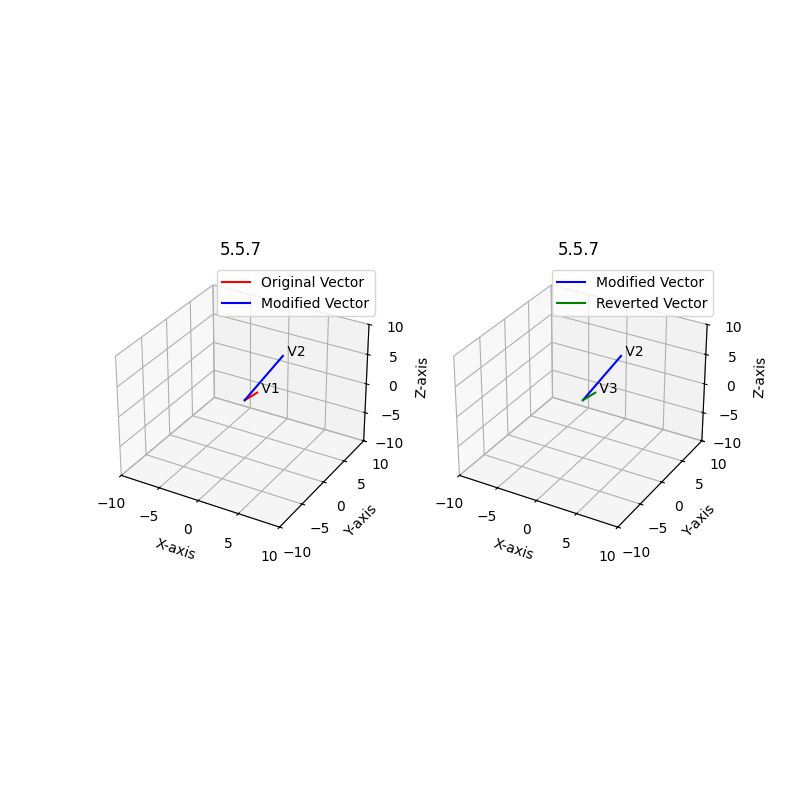
\includegraphics[width=0.8\columnwidth]{../figs/plot.png}
    \caption*{}
    \label{fig:plot}
\end{figure}
\end{frame}
\subsection{In pure Python}
\begin{frame}[fragile]{Pure Python code}
 \begin{lstlisting}[language=Python]
import numpy as np
import numpy.linalg as LA
import matplotlib.pyplot as plt

A = np.array([[3, 0, -1], [2, 3, 0], [0, 4, 1]])

x = np.array([1, 1, 1])
b = A @ x
c = LA.inv(A) @ b
print(x,A,b,c,sep='\n')


fig = plt.figure(figsize=(8, 8))
ax = fig.add_subplot(121, projection="3d")
\end{lstlisting}
\end{frame}
\begin{frame}[fragile]
\begin{lstlisting}[language=Python]
ax.quiver(0, 0, 0, x[0], x[1], x[2], color="red", label="Original Vector")
ax.text(x[0], x[1], x[2], " V1")
ax.quiver(0, 0, 0, b[0], b[1], b[2], color="blue", label="Modified Vector")
ax.text(b[0], b[1], b[2], " V2")

ax2 = fig.add_subplot(122, projection="3d")

ax2.quiver(0, 0, 0, b[0], b[1], b[2], color="blue", label="Modified Vector")
ax2.text(b[0], b[1], b[2], " V2")
ax2.quiver(0, 0, 0, c[0], c[1], c[2], color="green", label="Reverted Vector")
ax2.text(c[0], c[1], c[2], " V3")

\end{lstlisting}
\end{frame}
\begin{frame}[fragile]
\begin{lstlisting}[language=Python]
ax.set_xlabel("X-axis")
ax.set_ylabel("Y-axis")
ax.set_zlabel("Z-axis")
ax.set_title("5.5.7")
ax.set_xlim([-10, 10])
ax.set_ylim([-10, 10])
ax.set_zlim([-10, 10])
ax.legend()
ax.grid(True)
ax2.set_xlabel("X-axis")
ax2.set_ylabel("Y-axis")
ax2.set_zlabel("Z-axis")
ax2.set_title("5.5.7")
ax2.set_xlim([-10, 10])
ax2.set_ylim([-10, 10])
ax2.set_zlim([-10, 10])
ax2.legend()
ax2.grid(True)
plt.savefig("../figs/python.png")
plt.show()
\end{lstlisting}
\end{frame}
\subsection{Plot}
\begin{frame}{Plot}
 \begin{figure}[H]
    \centering
    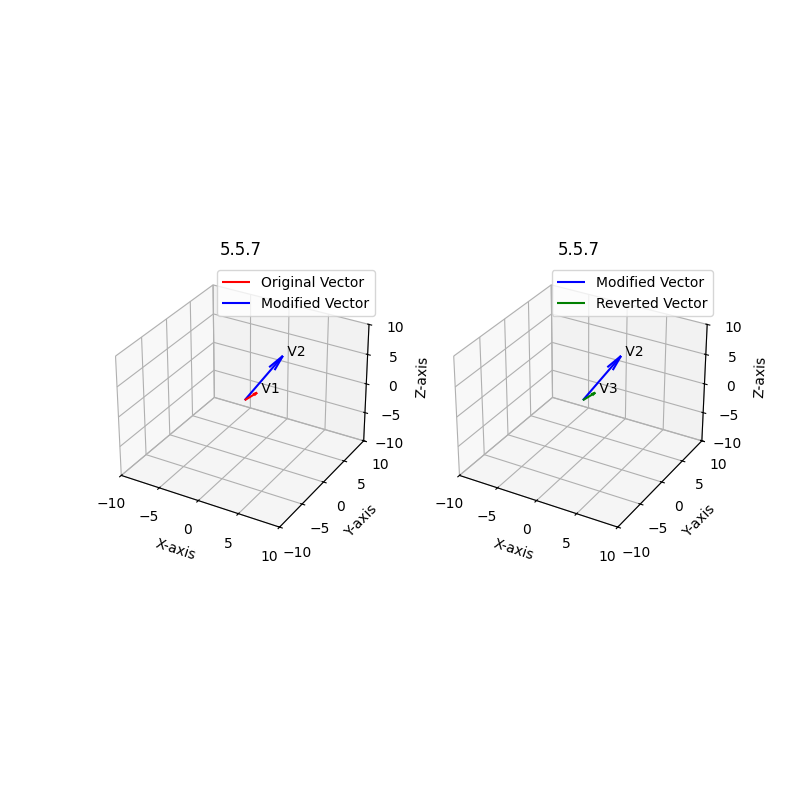
\includegraphics[width=0.75\columnwidth]{../figs/python.png}
    \caption*{}
    \label{fig:plot}
\end{figure}
\end{frame}
\end{document}
